% UC BERKELEY DEPARTMENT OF NUCLEAR ENGINEERING 
% ------------------------------------------------------------ 
% A page introducing students to the department.

\addcontentsline{toc}{section}{The Nuclear Engineering Department}
\section*{The Nuclear Engineering Department}
\begin{center}
  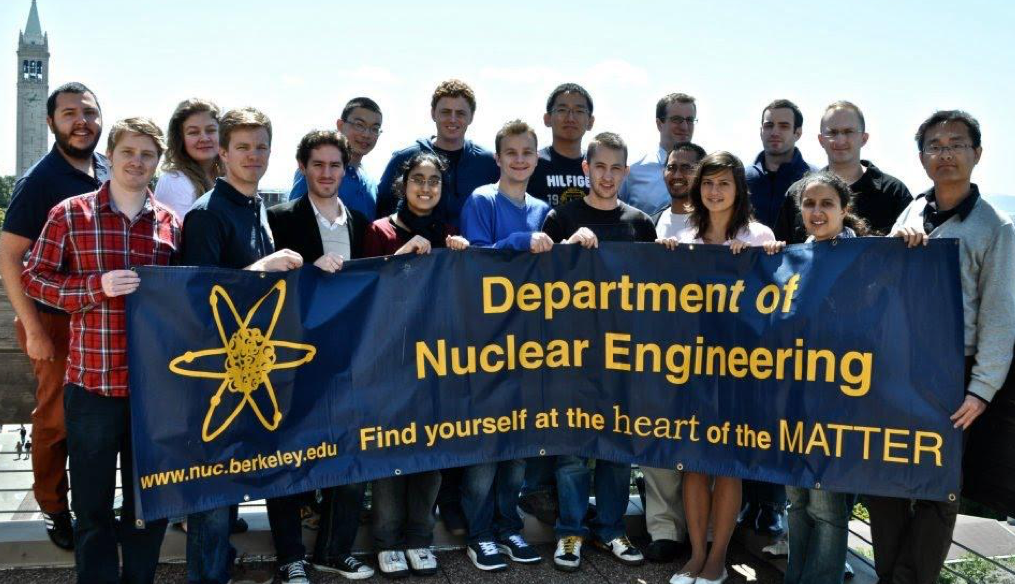
\includegraphics[width=\textwidth]{ne_department_old}
\end{center}

\vspace{0.25cm}
The Department of Nuclear Engineering was established in 1958. 
With close to 100 graduate students across several groups, the department offers a large variety of nuclear science and technology research while still feeling like a close community. 
Courses in the department range from traditional offerings in reactor theory and radiation detection to more unique classes and seminars focusing on nuclear materials and the physics of nuclear reactions. 
On top of those courses within the department, access to Berkeley's fantastic programs in physics, computer science, and chemistry allows Berkeley nuclear engineers to engage in an unparalleled level of interdisciplinary study and collaboration.

Beyond coursework, the department also has strong ties with several national laboratories and with industry.
Many Berkeley students actually perform their research at the local Lawrence Berkeley National Laboratory, while others work nearby at the Lawrence Livermore National Laboratory or the adjacent Sandia National Laboratory in Livermore, California (about a 40 minute drive). 
Though a bit further away, some students collaborate closely or have interned with advisors at Los Alamos, Oak Ridge, Argonne, and Idaho National Labs.
Finally, local advanced reactor start-ups Kairos and Oklo offer employment opportunities to Berkeley graduates in the Bay Area.
\vfill
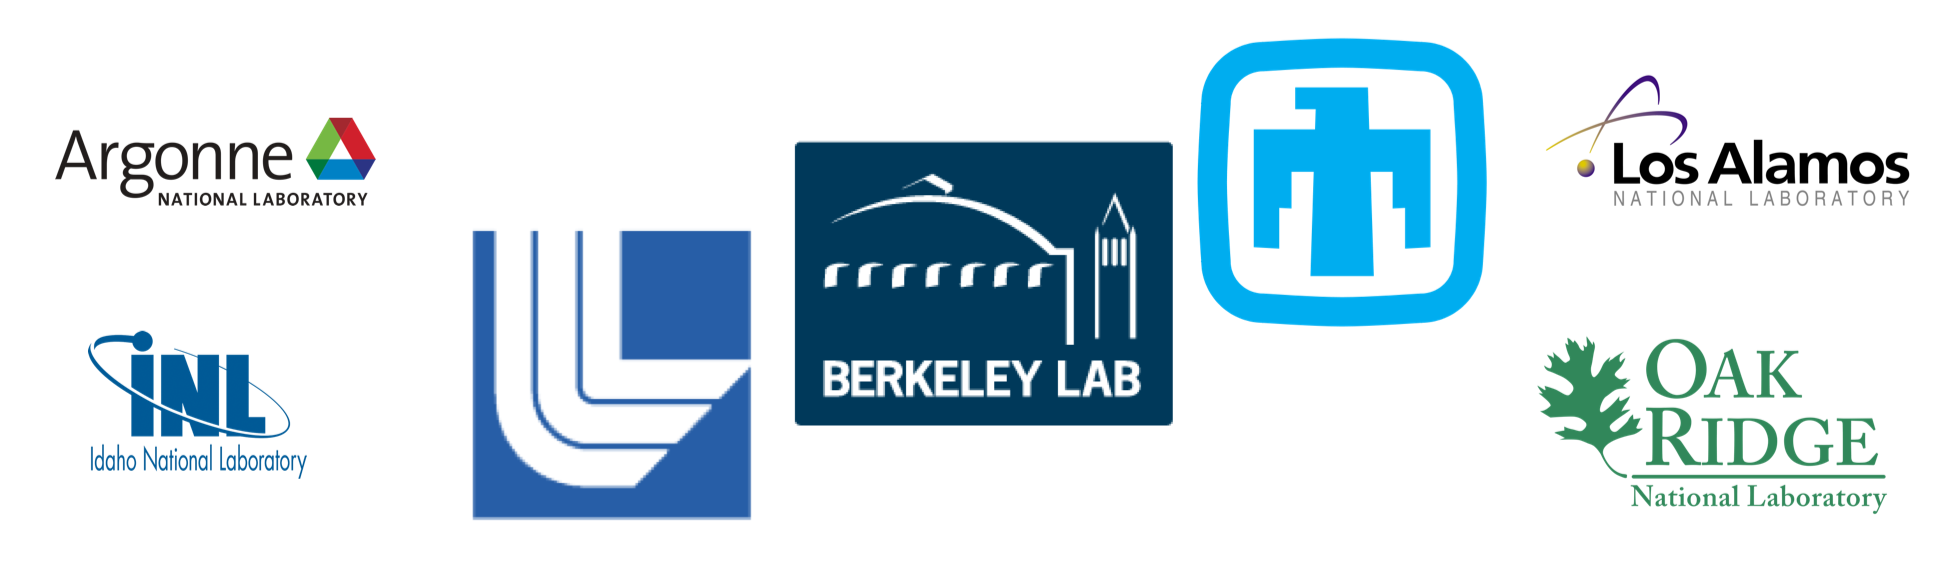
\includegraphics[width=16cm]{lab_logos}
